\chapter{Detecting Malicious Activity}
\label{detection}
Malicious activity is a generic term that refers to automated or
manual attempts of compromising the security of a computer
infrastructure. Examples of malicious activity include the output
generated (or its effect on a system) by the execution of simple
script kiddies, viruses, \ac{DoS} attacks, exploits of \ac{XSS} or
\ac{SQL} injection vulnerabilities, and so forth. This chapter
describes the research tools and methodologies available to detect and
mitigate malicious activity on a network, a single host, a web-server
and the combination of the three.

First, the background concepts and the \ac{ID} problem are described
in this chapter along with a taxonomic description of the most
relevant aspects of an \ac{IDS}. Secondly, a detailed survey of the
selected state-of-the-art anomaly detection approaches is presented
with the help of further classification dimensions. In addition, the
problem of alert correlation, that is an orthogonal topic, is
described and the most relevant, recent research approaches are
overviewed. Last but not least, the problem of evaluating an \ac{IDS}
is presented to provide the essential terminology and criteria to
understand the effectiveness of both the reviewed literature and our
original contributions.

\section{Intrusion Detection}
\label{detection:id}
\ac{ID} is the practice of analyzing a system to find malicious
activity. This section defines this concept more precisely by means of
simple but rigorous definitions. The context of such definitions is
the generic scenario of an Internet site, for instance, the network of
an \ac{ISP}. An example is depicted in
Figure~\ref{fig:ids-generic-scenario}. An Internet site ---and, in
general, the Internet itself--- is the state-of-the-art computer
infrastructure. In fact, it is a network that adopts almost any kind
of known computer technology (e.g., protocols, standards, containment
measures), it runs a rich variety of servers such as
\ac{HTTP}\index{HTTP}, \ac{FTP}\index{FTP}, \ac{SSH}\index{SSH},
\ac{VPN}\index{VPN} to support a broad spectrum of sophisticated
applications and services (e.g., web applications, e-commerce,
applications, the \textsf{Facebook Platform}, \textsf{Google
  Applications}). In addition, a generic Internet site receives and
process traffic from virtually any user connected to the Net and thus
represents the perfect research testbed for \ac{IDS}.

\begin{figure}[t]
  \centering
  \includegraphics[width=\textwidth]{figures/detection/ids-generic-scenario}
  \caption{Generic and comprehensive deployment scenario for
  \acp{IDS}\index{IDS}.}
  \label{fig:ids-generic-scenario}
\end{figure}

\begin{definition}[System]
  A \emph{system} is the domain of interest for security.
\end{definition}

\noindent Note that a system can be a physical or a logical one. For
instance, a physical system could be a host (e.g., the
\ac{DB}\index{DB} server or one of the client machines shown in the
figure), a whole network (e.g., the \ac{ISP} network shown in the
figure); a logical system can be an application, a service, such as
one of the web services run in a virtual machine deployed in the
\ac{ISP} network. While running, each system produces \emph{activity},
that we define as follows.

\begin{definition}[System activity]
  A system \emph{activity} is any data generated while the system is
  working. Such activity is formalized a sequence of events
  $\mathbb{I} = [I_{1}, I_{2}, I_{i}, \dots, I_{N}]$.
\end{definition}

\noindent For instance, each of the clients of
Figure~\ref{fig:ids-generic-scenario} produces system logs: in this
case $\mathbb{I}$ would contain an $I_{i}$ for each log entry. A human
readable representation follows.

\begin{logs} Aug 18 00:30:22 Adium[55011]: Warning: -[AIChatController
chatWithContact:(null)] got a nil targetContact.  Aug 18 00:29:40
[0x0-0x1b01b].org.mozilla.firefox[0]: NPP_Initialize called Aug 18
00:29:40 [0x0-0x1b01b].org.mozilla.firefox[0]: 2009-08-18 00:29:40.039
firefox-bin[254:10b] NPP_New(instance=0x169e0178,mode=2,argc=5) Aug 18
00:29:40 [0x0-0x1b01b].org.mozilla.firefox[0]: 2009-08-18 00:29:40.052
firefox-bin[254:10b] NPP_NewStream end=396239
\end{logs}

Similarly, the web servers generates \ac{HTTP}\index{HTTP} requests
and responses: in this case $\mathbb{I}$ would contain an $I_{i}$ for
each \ac{HTTP}\index{HTTP} message. Its human readable representation
follows.

\begin{logs} 128.111.48.4 [20/May/2009:15:25:42 -0700] "GET
/media//images/favicon.ico HTTP/1.0" 200 1150 "-" "Mozilla/5.0
(Macintosh; U; Intel Mac OS X 10.5; en-US; rv:1.9.0.10)
Gecko/2009042315 Firefox/3.0.10 Ubiquity/0.1.4" 128.111.48.4
[20/May/2009:15:26:44 -0700] "POST /report/ HTTP/1.0" 200 19171
"http://www.phonephishing.info/report/" "Mozilla/5.0 (Macintosh; U;
Intel Mac OS X 10.5; en-US; rv:1.9.0.10) Gecko/2009042315
Firefox/3.0.10 Ubiquity/0.1.4" 128.111.48.4 [20/May/2009:15:26:44
-0700] "GET /media//css/main.css HTTP/1.0" 200 5525
"http://www.phonephishing.info/report/" "Mozilla/5.0 (Macintosh; U;
Intel Mac OS X 10.5; en-US; rv:1.9.0.10) Gecko/2009042315
Firefox/3.0.10 Ubiquity/0.1.4" 128.111.48.4 [20/May/2009:15:26:44
-0700] "GET /media//css/roundbox.css HTTP/1.0" 200 731
"http://www.phonephishing.info/media//css/main.css" "Mozilla/5.0
(Macintosh; U; Intel Mac OS X 10.5; en-US; rv:1.9.0.10)
Gecko/2009042315 Firefox/3.0.10 Ubiquity/0.1.4"
\end{logs}

Other examples of system activity are described in Section
\ref{detection:id:taxonomy}.

In this document, we often used the term \emph{normal behavior}
referring to a set of characteristics (e.g., the distribution of the
characters of string parameters, the mean and standard deviation of
the values of integer parameters) extracted from the system activity
gathered during normal operation (i.e., without being
compromised). Moreover, in the remainder of this document, we need
other definitions.

\begin{definition}[Activity Profile]\label{def:activity-model}
  The \emph{activity profile} (or activity model) $c_{\mathbb{I}}$ is
  a set of models
  \begin{displaymath}
    c_{\mathbb{I}} = \langle m^{(1)}, \dots, m^{(u)}, \dots, m^{(U)}
    \rangle
  \end{displaymath} generated by extracting features from the system
  activity $\mathbb{I}$.
\end{definition}

\noindent This definition will be used in
Section~\ref{sec:misuse-vs-anomaly} and
Example~\ref{ex:misuse-vs-anomaly} and
\ref{ex:character-distribution-model} describe an instance of
$m^{(u)}$. An example of a real-world profile is described in
Example~\ref{ex:web-models}. We can now define the:

\begin{definition}[System Behavior]\label{def:system-behavior}
  The \emph{system behavior} is the set of features (or models), along
  with their numeric values, extracted by (or contained in) the
  activity profile.
\end{definition}

In particular, we will use this term as a synonym of \emph{normal}
system behavior, referring to the system behavior during normal
operation.

Given the high-accessibility of the Internet, publicly available
systems such as web servers, web applications, \ac{DB}\index{DB}
servers, are constantly at risk. In particular, they can be
compromised with the goal of stealing valuable information, deploying
infection kits or running phishing\index{phishing} and spam
campaigns. These are all examples of \emph{intrusions}. More formally.

\begin{definition}[Intrusion]
  An \emph{intrusion} is the automated or manual act of violating one
  or more security paradigms (i.e., confidentiality, integrity,
  availability) of a system. Intrusions are formalized as a sequence
  of events:

  \begin{displaymath}
    \mathbb{O} = [O_{1}, O_{2}, O_{i}, \dots, O_{M}] \subseteq
    \mathbb{I}
  \end{displaymath}
\end{definition}

\noindent Typically, when an intrusion takes place, a system behaves
unexpectedly and, as a consequence, its activity differs than during
normal operation. This is because an attack or the execution of
malware\index{malware} code often exploit vulnerabilities to bring the system into
states it was not designed for. For this reason, the activity that the
system generates is called \emph{malicious activity}; often, this term
is also used to indicate the attack or the malware\index{malware} code execution
itself. An example of $O_{i}$ is the following log entry: it shows
evidence of a \ac{XSS} attack that will make a vulnerable page to
display the arbitrary content supplied as part of the GET request
(while the page was not intentionally designed to this purpose).

\begin{logs} 128.111.48.4 [20/May/2009:15:29:44 -0700] "GET
/report/add/comment/<DIV
STYLE="background-image:\0075\0072\006C\0028'\006a\0061\0076\0061\0073\0063\0072\0069\0070\0074\003a\0061\006c\0065\0072\0074\0028.1027\0058.1053\0053\0027\0029'\0029">/
HTTP/1.0" 200 731 "http://www.phonephishing.info/report/add/"
"Mozilla/5.0 (Macintosh; U; Intel Mac OS X 10.5; en-US; rv:1.9.0.10)
Gecko/2009042315 Firefox/3.0.10 Ubiquity/0.1.4"
\end{logs}

\begin{note}
  We adopt a simplified representation of intrusions with respect to a
  dataset $\mathbb{D}$ (i.e., both normal and malicious): with
  $\mathbb{O} \subseteq \mathbb{D}$ we indicate that the activity
  $\mathbb{I}$ contains malicious events $\mathbb{O}$; however,
  strictly speaking, intrusions events and activity events can be of
  completely different types, thus the ''$\subseteq$'' relation may
  not be defined in a strict mathematical sense.
\end{note}

\noindent If a system is well-designed, any intrusion attempts always
leave some traces in the system's activity. These traces are called
\emph{tamper evidence} and are essential to perform \emph{intrusion
detection}.

\begin{definition}[Intrusion Detection]
  Intrusion \emph{detection} is the separation of intrusions from
  normal activity through the analysis of the activity of a system,
  while the system is running. Intrusions are marked as \emph{alerts},
  which are formalized as a sequence of event $\mathbb{A} = [A_{1},
  A_{2}, A_{i}, \dots, A_{L}] \subseteq \mathbb{O}$.
\end{definition}

\noindent Similarly, $\mathbb{A} \subseteq \mathbb{O}$ must not be
interpreted in a strict sense: it is just a notation to indicate that
for each intrusion, an alert may or may not exist. Note that \ac{ID}
can be also performed by manually inspecting a system activity. This
is clearly a tedious and unefficient task, thus research and
industrial interests are focused on automatic approaches.

\begin{definition}[Intrusion Detection System]
  An \emph{intrusion detection system} is an automatic tool that
  performs the \ac{ID} task.
\end{definition}

\noindent Given the above definitions, an abstract model of an
\ac{IDS} is shown in Figure~\ref{fig:ids-abstract-model}.

\begin{figure}[t]
  \centering
  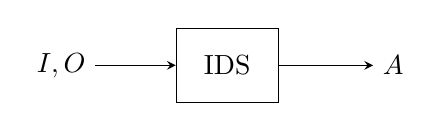
\begin{tikzpicture}[node distance=6em]
    \node (I) {$\mathbb{I}, \mathbb{O}$}; \node
    [draw,shape=rectangle,inner sep=1em] (ids) [right of=I] {IDS};
    \node (A) [right of=ids] {$\mathbb{A}$}; \draw[-stealth] (I) --
    (ids); \draw[-stealth] (ids) -- (A);
  \end{tikzpicture}
  \caption{Abstract I/O model of an \ac{IDS}.}
  \label{fig:ids-abstract-model}
\end{figure}

Although each \ac{IDS} relies on its own data model and format to
represent $\mathbb{A}$, the \ac{IETF} proposed \ac{IDMEF}
\citep{IDMEF} as a common format for reporting alert streams generated
by different \ac{IDS}.

\subsection{Evaluation}
\label{detection:evaluation} Evaluating an \ac{IDS} means running it
on collected data $\mathbb{D} = \mathbb{I} \cup \mathbb{O}$ that
resembles real-world scenarios. This means that such data includes
both intrusions $\mathbb{O}$ and normal activity $\mathbb{I}$, i.e.,
$|\mathbb{I}|, |\mathbb{O}| > 0$ and $\mathbb{I} \cap \mathbb{O} =
\varnothing$, i.e., $\mathbb{I}$ must include no malicious activity
other than $\mathbb{O}$.  The system is run in a controlled
environment to collect $\mathbb{A}$ along with performance indicators
for comparison with other systems. This section presents the basic
criteria used to evaluate modern \acp{IDS}\index{IDS}.

More precisely, to perform an evaluation experiment correctly a
fundamental hypothesis must hold: the set $\mathbb{O}$ must be known
and perfectly distinguishable from $\mathbb{I}$. In other words, this
means that, $\mathbb{D}$ must be labeled with a \emph{truth file},
i.e., a list of all the events known to be malicious. This allows to
treat the \ac{ID} problem as a classic classification problem, for
which a set of well-established evaluation metrics are available. In
particular, we are interested at calculating the following sets.

\begin{definition}[\acfp{TP}\index{TP}]
  The set of \emph{true positives} is $TP := \{A_{i} \in \mathbb{A}
  \mid \exists O_{j}: f(A_{i}) = O_{j}\}$.
\end{definition}

\noindent Where $f: \mathbb{A} \mapsto \mathbb{O}$ is a generic
function that, given an alert $A_{i}$ finds the corresponding
intrusion $O_{j}$ by parsing the truth file. The $TP$ set is basically
the set of alerts that are fired because a real intrusion has taken
place. The perfect \ac{IDS} is such that $TP \equiv \mathbb{O}$.

\begin{definition}[\acfp{TP}\index{TP}]
  The set of \emph{false positives} is
  \begin{displaymath}
    FP := \{A_{i} \in \mathbb{A} \mid \not\exists O_{j}: f(A_{i}) =
    O_{j}\}.
  \end{displaymath}
\end{definition}

\noindent On the other hand, the alerts in $FP$ are incorrect because
no real intrusion can be found in the observed activity. The perfect
\ac{IDS} is such that $FP = \varnothing$.

\begin{definition}[\acfp{TN}\index{TN}]
  The set of \emph{true negatives} is
  \begin{displaymath}
    TN := \{I_{j} \in \mathbb{I} \mid \not\exists A_{i}: f(A_{i}) =
    I_{j}\}.
  \end{displaymath}
\end{definition}

\noindent Note that the set of $TN$ does not contain
alerts. Basically, it is the set of correctly unreported alerts. The
perfect \ac{IDS} is such that $TN \equiv \mathbb{I}$.

\begin{definition}[\acfp{FN}\index{FN}]
  The set of \emph{false negatives} is
  \begin{displaymath}
    FN := \{O_{j} \in \mathbb{O} \mid \not\exists A_{i}: f(A_{i}) =
    O_{j}\}.
  \end{displaymath}
\end{definition}

\noindent Similarly to $TN$, $FN$ does not contain alerts. Basically,
it is the set of incorrectly unreported alerts. The perfect \ac{IDS}
is such that $FN = \varnothing$. Note that, $TP + TN + FP + TN = 1$
must hold.

In this and other documents, the term \emph{false alert} refers to $FN
\cup FP$. Given the aforementioned sets, aggregated measures can be
calculated.

\begin{definition}[\ac{DR}]
  The \emph{detection rate}, or \emph{true positive rate}, is defined
  as:

  \begin{displaymath}
    DR := \frac{TP}{TP + FN}.
  \end{displaymath}
\end{definition}

\noindent The perfect \ac{IDS} is such that $DR = 1$. Thus, the
\ac{DR} measures the detection capabilities of the system, that is,
the amount of malicious events correctly classified and reported as
alerts. On the other side, the \ac{FPR} is defined as follows.

\begin{definition}[\ac{FPR}]
  The \emph{false positive rate} is defined as:

  \begin{displaymath}
    FPR := \frac{FP}{FP + TN}.
  \end{displaymath}
\end{definition}

\noindent The perfect \ac{IDS} is such that $FPR = 0$. Thus, the
\ac{FPR} measures the inaccuracies of the system, that is, the amount
of legit events incorrectly classified and reported as alerts. There
are also other metrics such as the \emph{accuracy} and the
\emph{precision} which are often used to evaluate information
retrieval systems; however, these metrics are not popular for \ac{IDS}
evaluation.

\begin{figure}[tt]
  \centering
  \includegraphics[width=.8\textwidth]{figures/detection/roc-space}
  \caption{The \ac{ROC} space.}
  \label{fig:roc-space}
\end{figure}

The \ac{ROC} analysis, originally adopted to measure transmission
quality of radar systems, is often used to produce a compact and easy
to understand evaluation of classification systems. Even though there
is no standardized procedure to evaluate an \ac{IDS}, the research
community agrees on the use of \ac{ROC} curves to compare the
detection capabilities and quality of an \ac{IDS}. A \ac{ROC} curve is
the plot of $DR = DR(FPR)$ and is obtained by tuning the \ac{IDS} to
trade off \acp{FP}\index{FP} against true positives. Without going
into the details, each point of a \ac{ROC} curve correspond to a fixed
amount of $DR$ and $FPR$ calculated under certain conditions (e.g.,
sensitivity parameters). By modifying its configuration the quality of
the classification changes and other points of the \ac{ROC} are
determined. The \ac{ROC} space is plotted in
Figure~\ref{fig:roc-space} along with the performances of a random
classifiers, characterized by $DR = FPR$. The perfect, ideal \ac{IDS}
can increase its $DR$ from 0 to 1 with $FPR = 0$: however, it must
hold that $FPR \to 1 \Rightarrow DR \to 1$.

\subsection{Alert Correlation}
\label{detection:id:alert-correlation} The problem of intrusion
detection is challenging in todays' complex networks. In fact, it is
common to have more than one \ac{IDS}\index{IDS} deployed, monitoring
different segments and different aspects of the whole infrastructure
(e.g., hosts, applications, network, etc.). The amount of alerts
reported by a network of \acp{IDS}\index{IDS} running in a complex
computer infrastructure is larger, by several orders of magnitude,
than what was common in the smaller networks monitored years ago. In
such a context, network administrators are loaded by several alerts
and long security reports often containing a non-negligible amount of
\acp{FP}\index{FP}. Thus, the creation of a clean, compact, and
unified view of the security status of the network is needed. This
process is commonly known as alert correlation
\citep{valeur04comprehensive} and it is currently one of the most
difficult challenges of this research field. More precisely.

\begin{definition}[Alert Correlation]
  The \emph{alert correlation} is the identification of relations
  among alerts

  \begin{displaymath}
    A_{1}, A_{2}, A_{i}, \dots, A_{L} \in \mathbb{A}_{1} \cup
    \mathbb{A}_{2} \cup \cdots \cup \mathbb{A}_{K}
  \end{displaymath}

  to generate a unique, more compact and comprehensive sequence of
  alerts $\mathbb{A'} = [A'_{1}, A'_{2}, \dots, A'_{P}]$.
\end{definition}

A desirable property is that $\mathbb{A}'$ should be as complete as
$\mathbb{A}_{1} \cup \mathbb{A}_{2} \cup \cdots \cup \mathbb{A}_{K}$
without introducing errors such as alerts that do not correspond to a
real intrusion. As for the \ac{ID}, alert correlation can be a manual,
and tedious, task. Clearly, automatic alert correlation systems are
more attractive and can be considered a complement of a modern
\ac{IDS}.

\begin{definition}[Alert Correlation System]
  An \emph{alert correlation system} is an automatic tool that
  performs the alert correlation task.
\end{definition}

\noindent The overall \ac{IDS} abstract model is complemented with an
alert correlation engine as shown in
Figure~\ref{fig:ids-ac-abstract-model}.

\begin{figure}[t]
  \centering
  \begin{tikzpicture}[node distance=6em]
    \node (I) {$\mathbb{I}, \mathbb{O}$}; \node
    [draw,shape=rectangle,inner sep=1em,double copy shadow,fill=white]
    (ids) [right of=I] {IDS}; \node (A) [right of=ids,text
    width=1.2em] {$\mathbb{A}_{1}$\\...\\$\mathbb{A}_{n}$}; \node
    [draw,shape=rectangle,inner sep=1em,fill=white] (acs) [right of=A]
    {ACS}; \node (Ap) [right of=acs] {$\mathbb{A}'$}; \draw[-stealth]
    (I) -- (ids); \draw[-stealth] (ids) -- (A); \draw[-stealth] (A) --
    (acs); \draw[-stealth] (acs) -- (Ap);
  \end{tikzpicture}
  \caption{Abstract I/O model of an \ac{IDS} with an alert correlation
  system.}
  \label{fig:ids-ac-abstract-model}
\end{figure}

\subsection{Taxonomic Dimensions}
\label{detection:id:taxonomy}
The first comprehensive taxonomy of \acp{IDS}\index{IDS} has been
proposed in \citep{debar1999towards} and revised in
\citep{debar2000revised}. Another good survey appeared in
\citep{axelsson-intrusion}.

Compared to the classic survey found in the literature, this section
complements the basic taxonomic dimensions by focusing on
\emph{modern} techniques. In particular, todays' intrusion detection
approaches can be categorized by means of the specific modeling
techniques appeared in recent research.

It is important to note that the taxonomic dimensions that are
hereby suggested are not exhaustive, thus certain \acp{IDS} may not
fit into it (e.g.,
\citep{vigilante,argos:eurosys06,newsome2005dynamic}). On the other
hand, an exhaustive and detailed taxonomy would be difficult to
read. To overcome this difficulty, in this section we describe a
high-level, technique-agnostic taxonomy based on the dimensions
summarized in Table~\ref{tab:misuse-vs-anomaly}; in each sub-section
of Section~\ref{detection:ad}, which focus on anomaly-based models, we
expand the taxonomic dimensions by listing and accurately detailing
further classification criteria.

\subsubsection{Type of model}
\label{sec:misuse-vs-anomaly} \acp{IDS}\index{IDS} must be divided
into two opposite groups: misuse\hyp{}based \emph{vs.}
anomaly\hyp{}based. The former create models of the \emph{malicious}
activity while the latter create models of \emph{normal}
activity. Misuse-based models look for \emph{patterns} of malicious
activity; anomaly-based models look for \emph{unexpected} activity. In
some sense, \acp{IDS}\index{IDS} can either ``blacklist'' or
``whitelist'' the observed activity.

Typically, the first type of models consists in a database of all the
known attacks. Besides requiring frequent updates ---which is just a
technical difficulty and can be easily automated--- misuse-based
systems assumes the feasibility of enumerating \emph{all} the
malicious activity.

Despite the limitation of being inherently incomplete, misuse-based
systems widely adopted in the real-world
\citep{snortlisa,snortsite}. This is mainly due to their simplicity
(i.e., attack models are triggered by means of pattern matching
algorithms) and accuracy (i.e., they generate virtually no false
alerts because an attack signature can either match or not).

Anomaly-based approaches are more complex because creating a
specification of normal activity is obviously a difficult task. For
this reason, there are no well-established and widely-adopted
techniques; instead, misuse models are as sophisticated as a pattern
matching problem. In fact, the research on anomaly-based systems is
very active.

These systems are effective only under the assumption that malicious
activity, such as an attack or malware\index{malware} being executed, \emph{always}
produces sufficient deviations from normal activity such that models
are triggered, i.e., anomalies. This clearly has the positive
side-effect of requiring zero knowledge on the malicious activity,
which makes these systems particularly interesting. The negative
side-effect is their tendency of producing a significant amount of
false alerts (the notion of ``significant amount of false alerts''
will be discussed in detail in Section
\ref{detection:evaluation:base-rate-fallacy}).

Obviously, an \ac{IDS} can benefit of both the techniques by, for
instance, enumerating all the known attacks and using anomaly-based
heuristics to prompt for suspicious activity. This practice is often
adopted by modern anti-viruses.

It is important to remark that, differently from the other taxonomic
dimensions, the distinction between misuse- and anomaly-based
approaches is fundamental: they are based on opposite hypotheses and
yield to completely different system designs and results. Their
duality is highlighted in Table \ref{tab:misuse-vs-anomaly}.

\begin{table}[t]
  \centering
  \begin{tabular}{rcc}
    \toprule \emph{Feature} & \textsc{Misuse-based} &
    \textsc{Anomaly-based}\\
    
    \midrule Modeled activity: & Malicious &
    Normal\\
    
    Detection method: & Matching & Deviation\\

    Threats
    detected: & Known & Any\\

    False negatives: & High & Low\\

    False
    positives: & Low & High\\

    Maintenance cost: & High & Low\\ Attack
    desc.: & Accurate & Absent\\

    System design: & Easy & Difficult\\
    \bottomrule
  \end{tabular}
  \caption{Duality between misuse- and anomaly-based intrusion
    detection techniques. Note that, an anomaly-based \ac{IDS} can
    detect ``Any'' threat, under the assumption that an attack always
    generates a deviation in the modeled activity.}
  \label{tab:misuse-vs-anomaly}
\end{table}

\begin{example}[Misuse \emph{vs.} Anomaly]\label{ex:misuse-vs-anomaly}
  A misuse-based system $M$ and an anomaly-based system $A$ process
  the same log containing a full dump of the system calls invoked by
  the kernel of an audited machine. Log entries are in the form:

  \begin{center}\small
    \begin{verbatim} <function_name>(<arg1_value>, <arg2_value>, ...)
    \end{verbatim}
  \end{center}

\noindent The system $M$ has the following simple attack
model\footnote{Generated from the real world exploit
\url{http://milw0rm.com/exploits/9303}}:

\begin{pseudoc}
  if (function_name == "read") {
    /* ... */ if (match(decode(arg3_value), "a{4}b{4}c{4}d{4}e{4}\
        f{4}...x{4}3RH~TY7{33}QZjAXP0A0AkAAQ2AB2BB0BBAB\
        XP8ABuJIXkweaHrJwpf02pQzePMhyzWwSuQnioXPOHuBxKn\
        aQlkOjpJHIvKOYokObPPwRN1uqt5PA..." ))
    fire_alert("VLC bug 35500 is being exploited!"); /* ... */
  }
\end{pseudoc}
\end{example}

The simple attack signature looks for a pattern generated from the
exploit. If the content of the buffer (i.e., \texttt{arg3\_value})
that stores the malicious file matches the given pattern then an alert
is fired.

\noindent On the other hand, the system $A$ has the following model,
based on the sample character distribution of each file's
content. Such frequencies are calculated during normal operation of
the application.

\begin{pseudoc}
  /* ... */ cd['<'] = {0.1, 0.11} cd['a'] = {0.01, 0.2} cd['b'] =
  {0.13, 0.23} /* ... */

  b = decode(arg3_value);
  
  if ( !(cd['c'][0] < count('c', b) < cd['c'][1]) ||\
       !(cd['<'][0] < count('<', b) < cd['<'][1]) ||\
       ... || ...)  fire_alert("Anomalous content detected!");
  /* ... */
\end{pseudoc}

Obviously, more sophisticated models can be designed. The purpose of
this example is that of highlighting the main differences between the
two approaches.

\medskip

A generalization of the aforementioned examples allows us to better
define an anomaly-based \ac{IDS}.

\begin{definition}[Anomaly-based \ac{IDS}]
  An \emph{anomaly-based \ac{IDS}} is a type of \ac{IDS} that generate
  alerts $\mathbb{A}$ by relying on normal activity profiles
  (Definition~\ref{def:activity-model}).
\end{definition}

\subsubsection{System activity} \acp{IDS}\index{IDS} can be classified
based on the type of the activity they monitor. The classic literature
distinguishes between network\hyp{}based and host\hyp{}based systems;
\ac{NIDS} and \ac{HIDS}, respectively. The former inspect network
traffic (i.e., raw bytes sniffed from the network adapters), and the
latter inspect the activity of the operating system. The scope of a
network-based system is as large as the broadcast domain of the
monitored network. On the other hand, the scope host-based systems is
limited to the single host.

Network-based \acp{IDS}\index{IDS} have the advantage of having a
large scope, while host-based ones have the advantage of being fed
with detailed information about the host they run on (e.g., process
information, \ac{CPU}\index{CPU} load, number of active processes,
number of users). This information is often unavailable to
network-based systems and can be useful to refine a decision regarding
suspicious activity. For example, by inspecting both the network
traffic and the kernel activity, an \ac{IDS} can filter the alerts
regarding the \textsf{Apache} web server version 2.0.0 on all the
hosts running version 2.0.2. On the other hand, network-based systems
are centralized and are much more easy to manage and deploy. However,
\ac{NIDS} are limited to the inspection of unencrypted payload, while
\ac{HIDS} may have it decrypted by the application layer. For example,
a \ac{NIDS} cannot detect malicious HTTPS traffic.

The network stack is standardized (see
Note~\ref{note:network-stack-standardized}), thus the definition of
network-based \ac{IDS} is precise. On the other hand, because of the
immense variety of operating system implementations, a clear
definition of ``host data'' lacks. Existing host-based
\acp{IDS}\index{IDS} analyze audit log files in several formats, other
systems keep track of the commands issued by the users through the
console. Some efforts have been made to propose standard formats for
host data: \ac{BSM}\index{BSM} and its modern re-implementation called
\textsf{OpenBSM} \citep{openbsm,openbsm_site} are probably the most
used by the research community as they allow developers to gather the
full dump of the system calls before execution in the kernel.

\begin{note}\label{note:network-stack-standardized}
  Although the network stack implementation may vary from system to
  system (e.g., \textsf{Windows} and \textsf{Cisco} platforms have
  different implementation of \ac{TCP}), it is important to underline
  that the notion of IP, TCP, HTTP \emph{packet} is well defined in a
  system-agnostic way, while the notion of \emph{operating system
    activity} is rather vague and by no means standardized.
\end{note}

Example \ref{ex:misuse-vs-anomaly} describes a sample host-based
misuse detection system that inspects the arguments of the system
calls. A similar, but more sophisticated, example based on network
traffic is \textsf{Snort} \citep{snortlisa,snortsite}.

\begin{note}[Inspection layer]
  Network-based systems can be further categorized by their protocol
  inspection capabilities, with respect to the network
  stack. \webanomaly \citep{kruegel:jcn2005:webanomaly,webanomalysite}
  is network\hyp{}based, in the sense that runs in promiscuous mode
  and inspects network data. On the other hand, it also
  \ac{HTTP}\index{HTTP}-based, in the sense that decodes the payload
  and reconstructs the \ac{HTTP}\index{HTTP} messages (i.e., request
  and response) to detect attacks against web applications.
\end{note}

\subsubsection{Model construction method} Regardless of their type,
misuse- or anomaly-based, models can be specified either manually or
automatically. However, for their nature, misuse models are often
manually written because they are based on the exhaustive enumeration
of known malicious activity. Typically, these models are called attack
signatures; the largest repository of manually generated misuse
signatures is released by the \textsf{Sourcefire Vulnerability
Research Team\texttrademark} \citep{snortrules}. Misuse signatures can
be generated automatically: for instance, in \citep{1251258} a method
to build misuse models of worms is described. Similarly,
low-interaction honeypots often uses malware\index{malware} emulation to
automatically generate signatures. Two recently proposed techniques
are \citep{argos:eurosys06,1224380}.

On the other hand, anomaly-based models are more suitable for
automatic generation. Most of the anomaly-based approaches in the
literature focus on unsupervised learning mechanisms to construct
models that precisely capture the normal activity observed. Manually
specified models are typically more accurate and are less prone to
\acp{FP}\index{FP}, although automatic techniques are clearly more
desirable.

\begin{example}[Learning character
distributions]\label{ex:character-distribution-model}
  In Example \ref{ex:misuse-vs-anomaly}, the described system $A$
  adopts a learning based character distribution model for
  strings. Without going into the details, the idea described in
  \citep{mutz06:syscalls} observes string arguments and estimate the
  characters' distribution over the \ac{ASCII}\index{ASCII} set. More
  practically, the model is a histogram $H(c), \forall c \in {0,
  255}$, where $H(c)$ is the normalized frequency of character
  $c$. During detection, a $\chi^{2}$ test is used to decide whether
  or not a certain sting is deemed anomalous.

Beside the obvious advantage of being resilient against evasion, this
model requires no human intervention.
\end{example}

\section{Relevant Anomaly Detection Techniques}
\label{detection:ad} Our research focuses on anomaly detection. In
this section, the selected state of the art approaches are reviewed
with particular attention to network\hyp{}, host\hyp{} and
web\hyp{}based techniques, along with the most influential approaches
in the recent literature alert correlation. This section provides the
reader with the basic concepts to understand our contributions.

\subsection{Network-based techniques}
\label{detection:ad:network}
Our research does not include network-based \acp{IDS}\index{IDS}. Our
contributions in alert correlation, however, leverage both network-
and host-based techniques, thus a brief overview of the latest (i.e.,
proposed between 2001 and 2006) network-based detection approaches is
provided in this section. We remark that all the techniques included
in the following are based on \ac{TCP}\index{TCP}/IP, meaning that
models of normal activity are constructed by inspecting the decoded
network frames up to the \ac{TCP}\index{TCP} layer.

In Table \ref{tab:network-sota-taxonomy} the selected approaches are
marked with bullets to highlight their specific characteristics. Such
characteristics are based on our analysis and experience, thus, other
classifications may be possible. They are defined as follows:

\begin{description}
\item[Time] refers to the use of \emph{timestamp} information,
extracted from network packets, to model normal packets. For example,
normal packets may be modeled by their minimum and maximum
inter-arrival time.
\item[Header] means that the \ac{TCP}\index{TCP} header is decoded and
the fields are modeled. For example, normal packets may be modeled by
the observed ports range.
\item[Payload] refers to the use of the payload, either at
\ac{IP}\index{IP} or \ac{TCP}\index{TCP} layer. For example, normal
packets may be modeled by the most frequent byte in the observed
payloads.
\item[Stochastic] means that stochastic techniques are exploited to
create models. For example, the model of normal packets may be
constructed by estimating the sample mean and variance of certain
features (e.g., port number, content length).
\item[Deterministic] means that certain features are modeled following
a deterministic approach. For example, normal packets may be only
those containing a specified set of values for the \ac{TTL}\index{TTL}
field.
\item[Clustering] refers to the use of clustering (and subsequent
classification) techniques. For instance, payload byte vectors may be
compressed using a \ac{SOM} where class of different packets will
stimulate neighbor nodes.
\end{description}

Note that, since recent research have experimented with several
techniques and algorithms, mixed approaches exist and often lead to
better results.

\begin{sidewaystable}
  \renewcommand{\arraystretch}{1.5} \centering
  \begin{tabular}{rcccccc}
    \toprule \textsc{Approach} & \textsc{Time} & \textsc{Header} &
    \textsc{Payload} & \textsc{Stochastic} & \textsc{Determ.} &
    \textsc{Clustering}\\

    \midrule \citep{phad} & & $\bullet$ & & & &
    $\bullet$ \\

    \citep{kruegel:sac2002:anomaly} & & $\bullet$ &
    $\bullet$ & $\bullet$ & & \\

    \citep{protocolanom} & & $\bullet$ &
    & $\bullet$ & $\bullet$ & \\

    \citep{ramadas} & & & $\bullet$ & & &
    $\bullet$ \\

    \citep{rules-payl} & $\bullet$ & & $\bullet$ & &
    $\bullet$ & \\

    \citep{zanero-savaresi} & & $\bullet$ & $\bullet$ &
    & & $\bullet$ \\

    \citep{wang:raid2004:payl} & & & $\bullet$ &
    $\bullet$ & & \\

    \citep{zanero-pattern} & & $\bullet$ & $\bullet$
    & & & $\bullet$ \\

    \citep{DBLP:conf/iwia/BolzoniEHZ06} & & $\bullet$ & $\bullet$
    & & & $\bullet$ \\

    \citep{wang:raid2006:anagram} & & & $\bullet$ &
    $\bullet$ & & \\

 \bottomrule
  \end{tabular}
  \caption{Taxonomy of the selected state of the art approaches for
    network-based anomaly detection.}
  \label{tab:network-sota-taxonomy}
\end{sidewaystable}

In~\citep{phad} a mostly deterministic, simple detection technique is
presented. During training, each field of the header of the \ac{TCP}
packets are extracted and tokenized into 4 bytes bins (for memory
efficiency reasons). The tokenized values are clustered by means of
their values and every time a new value is observed the clustering is
updated. The detection approach is deterministic, since a packet is
classified as anomalous if the values of its header do not match any
of the clusters. Besides the fact of being completely unsupervised,
this techniques detects between 50\% and 75\% of the probe and
\ac{DoS} attacks, respectively, in \ac{IDEVAL} 1999
\citep{ideval_1999_doc}. Slight performance issues and a rate of 10
\acp{FP}\index{FP} per day (i.e., roughly, 1 false alert every 2
hours) are the only disadvantage of the approach.

The approach described in~\citep{kruegel:sac2002:anomaly} reconstructs
the payload stream for each service (i.e., port); this avoids to evade
the detection mechanism by using packet fragmentation. In addition to
this, a basic application inspection is performed to distinguish among
the different types of request of the specific service, e.g., for
\ac{HTTP}\index{HTTP} the service type could be GET, POST, HEAD. The
sample mean and variance of the content length are also calculated and
the distribution of the bytes (interpreted as \ac{ASCII}\index{ASCII}
characters) found in the payload is estimated using simple
histograms. The anomaly score used for detection aggregates
information regarding the type of service, expected content length and
payload distribution. With a low performance overhead and low
\ac{FPR}, this system is capable of detecting anomalous interactions
with the application layer. One critique is that the system has not
been tested on several applications other than \ac{DNS}\index{DNS}.

Probably inspired by the misuse-based, finite-state technique
described in~\citep{vigna:1999:netstat}, in \citep{protocolanom} the
authors describe a system to learn the \ac{TCP} specification. The
basic finite state model is extended with a network of stochastic
properties (e.g., the frequency of certain transitions, the most
common value of a state attribute, the distribution of the values
found in the fields of the \ac{IP} packets) among states and
transitions. Such properties are estimated during training and
exploited at detection to implement smoother thresholds that ensure as
low as 5.5 false alerts per day. On the other hand, the deterministic
nature of the finite state machine detects attacks with a 100\%
\ac{DR}.

\ac{LERAD}, the system described in~\citep{rules-payl} is an optimized
rule mining algorithm that works well on data with tokenized domains
such as the fields of \ac{TCP}\index{TCP} or \ac{HTTP}\index{HTTP}
packets. Although the idea implemented in \ac{LERAD} can be applied at
any protocol layer, it has been tested on \ac{TCP} and \ac{HTTP} but
no more than the 64\% of the attack in the testing dataset were
detected. Even if the \ac{FPR} is acceptable (i.e., 10 alerts per day)
its limited detection capabilities worsen if real-world data is used
instead of synthetic datasets such as \ac{IDEVAL}. In
\citep{rulessystemcallarguments} the \ac{LERAD}\index{LERAD} algorithm
(Learning Rules for Anomaly Detection) is used to mine rules
expressing ``normal'' values of arguments, normal sequences of system
calls, or both. No relationship is learned among the values of
different arguments; sequences and argument values are handled
separately; the evaluation is quite poor however, and uses
non-standard metrics.

Unsupervised learning techniques to mine pattern from payload of
packets has been shown to be an effective approach. Both the
network-based approaches described so far and other proposals
\citep{nsom,NETAD} had to cope with data represented using a high
number of dimensions (e.g., a vector with 1460 dimensions, that is the
maximum number of bytes in the \ac{TCP}\index{TCP} payload). While the
majority of the proposals circumvent the issue by ignoring the
payload, the aforementioned issue is brilliantly solved in
\citep{ramadas} and extended in \ac{ULISSE}
\citep{zanero-savaresi,zanero-pattern} by exploiting the clustering
capabilities of a \ac{SOM} \citep{bibbiasom} with a faster algorithm
\citep{zanero-speedup}, specifically designed for high-dimensional
data. The payload of \ac{TCP} packets is indeed compressed into the
bi-dimensional grid representing the \ac{SOM}, organized in such a way
that class of packets can be quickly extracted. The approach relies
on, and confirms, the assumption that the traffic belongs to a
relatively small number of services and protocols that can be mapped
onto a small number of clusters. Network packet are modeled as a
multivariate time-series, where the variables include the packet class
into the \ac{SOM} plus some other features extracted from the
header. At detection, a fast discounting learning algorithm for
outlier detection \citep{smartsifter} is used to detect anomalous
packets. Although the system has not been released yet, the prototype
is able to reach a 66.7\% \ac{DR} with as few as 0.03\%
\acp{FP}\index{FP}. In comparison, one of the prototype dealing with
payloads available in literature \citep{wang:raid2005:payl}, the best
overall result leads to the detection of 58.7\% of the attacks, with a
\ac{FPR} that is between 0.1\% and 1\%. The main weakness of this
approach is that it works at the granularity of the packets and thus
might be prone to simple evasion attempts (e.g., by splitting an
attack onto several malicious packets, interleaved with long sequence
of legit packets). Inspired by~\citep{wang:raid2005:payl}
and~\citep{zanero-savaresi}, \citep{DBLP:conf/iwia/BolzoniEHZ06} has
been proposed.

The approach presented in~\citep{wang:raid2005:payl} differs from the
one described in~\citep{zanero-savaresi,zanero-pattern} even though
the underlying key idea is rather similar: byte frequency
distribution. Both the two approaches, and
also~\citep{kruegel:sac2002:anomaly}, exploit the distribution of byte
values found in the network packets to produce some sort of
``normality'' signatures. \citep{wang:raid2005:payl} utilizes a simple
clustering algorithm to aggregate similar packets and produce a
smoother and more abstract signature,
\citep{zanero-savaresi,zanero-pattern} introduces the use of \ac{SOM}
to accomplish the task of finding classes of normal packets.

An extension to~\citep{wang:raid2004:payl}, which uses $1$-grams, is
described in~\citep{wang:raid2006:anagram} that uses higher-order,
randomized $n$-grams to mitigate mimicry attacks. In addition, the
newer approach does not estimate the frequency distribution of the
$n$-grams, which causes many \acp{FP}\index{FP} if $n$
increases. Instead, it adopts a filtering technique to compress the
$n$-grams into memory efficient arrays of bits. This decreased the
\ac{FPR} of about two orders of magnitude.

\subsection{Host-based techniques}
\label{detection:ad:host} A survey of the latest (i.e., proposed
between 2000 and 2009) host-based detection approaches is provided in
this section. Most of the techniques leverage system call invoked by
the kernel to create models of normal behavior of processes.

In Table \ref{tab:host-sota-taxonomy} the selected approaches are
marked with bullets to highlight their specific characteristics. Such
characteristics are based on our analysis and experience, thus, other
classifications may be possible. They are defined as follows:

\begin{description}
\item[Syscall] refers, in general, to the use of system calls to
characterize normal host activity. For example, a process may be
modeled by the stream of system calls invoked during normal operation.
\item[Stochastic] means that stochastic techniques are exploited to
create models. For example, the model of normal processes may be
constructed by estimating the sample mean and variance of certain
features (e.g., length of the \texttt{open}'s \texttt{path} argument).
\item[Deterministic] means that certain features are modeled following
a deterministic approach. For example, normal processes may be only
those that use a fixed number, say 12, of file descriptors.
\item[Comprehensive] approaches are those that have been extensively
developed and, in general, incorporate a rich set of features, beyond
the proof-of-concept.
\item[Context] refers to the use of context information in
general. For example, the normal behavior of processes can be modeled
also by means of the number of the environmental variables utilized or
by the sequence of system calls invoked.
\item[Data] means that the data flow is taken into account. For
example, normal processes may be modeled by the set of values of the
system call arguments.
\item[Forensics] means that the approach has been also evaluated for
off-line, forensics analysis.
\end{description}

Our contributions are included in Table \ref{tab:host-sota-taxonomy}
and are detailed in Chapter \ref{host}. Note that, since recent
research have experimented with several techniques and algorithms,
mixed approaches exist and often lead to better results.

\begin{sidewaystable}
  \renewcommand{\arraystretch}{1.3}
  \centering\footnotesize
  \begin{tabular}{rcccccccc}
    \toprule \textsc{Approach} & \textsc{Syscall} & \textsc{Determ.} &
    \textsc{Stochastic} & \textsc{Comprehen.} & \textsc{Context} &
    \textsc{Data} & \textsc{Forensics} \\

    \midrule

    \citep{lee:2000:framework} & & & $\bullet$ & $\bullet$ & & & \\

    \citep{sekar:sp2001:automaton} & $\bullet$ & $\bullet$ & & & & &
    \\

    \citep{wagner:sp2001:staticanalysis} & $\bullet$ & $\bullet$ &
    & & & & \\

    \citep{rulessystemcallarguments} & $\bullet$ &
    $\bullet$ & & & $\bullet$ & & \\

    \citep{libanomaly} & $\bullet$ &
    & $\bullet$ & $\bullet$ & $\bullet$ & $\bullet$ & \\

    \citep{zanero-ethology} & $\bullet$ & & $\bullet$ & & $\bullet$ &
    & \\

    \citep{giffin} & $\bullet$ & $\bullet$ & & & $\bullet$ &
    $\bullet$ & \\

    \citep{mutz06:syscalls} & $\bullet$ & & $\bullet$ &
    $\bullet$ & & $\bullet$ & \\

    \citep{venkat_dataflow} & $\bullet$ &
    $\bullet$ & & & $\bullet$ & $\bullet$ & \\

    \citep{mutz:raid2007:syscalls} & $\bullet$ & & $\bullet$ &
    $\bullet$ & & $\bullet$ & \\

    \citep{1352621} &
    $\bullet$ & $\bullet$ & & & $\bullet$ & $\bullet$ & \\

    \textbf{\citep{zanero_self}} &
    $\bullet$ & & $\bullet$ & & $\bullet$ & $\bullet$ & $\bullet$ \\

    \textbf{\citep{10.1109/TDSC.2008.69}} & $\bullet$ & & $\bullet$ &
    $\bullet$ & $\bullet$ & $\bullet$ & \\

    \textbf{\citep{2009_frossi_maggi_rizzo_zanero_improving_syscall_models}}
    & $\bullet$ & $\bullet$ &
    $\bullet$ & & $\bullet$ & $\bullet$ & \\

    \bottomrule
  \end{tabular}
  \caption{Taxonomy of the selected state of the art approaches for
    host-based anomaly detection. Our contributions are highlighted.}
  \label{tab:host-sota-taxonomy}
\end{sidewaystable}

Host-based anomaly detection has been part of intrusion detection
since its very inception: it already appears in the seminal
work~\citep{anderson}. However, the definition of a set of statistical
characterization techniques for events, variables and counters such as
the \ac{CPU}\index{CPU} load and the usage of certain commands is due
to~\citep{denning:tse1987:ides}. The first mention of intrusion
detection through the analysis of the sequence of syscalls from system
processes is in \citep{Self}, where ``normal sequences'' of system
calls are considered. A similar idea was presented earlier in
\citep{PrivilegedProgramsMonitoring}, which proposes a misuse-based
idea by manually describe the canonical sequence of calls of each and
every program, something evidently impossible in practice.

In \citep{lee:2000:framework} a set of models based on data mining
techniques is proposed. In principle, the models are agnostic with
respect to the type of raw event collected, which can be user activity
(e.g., login time, \ac{CPU}\index{CPU} load), network packets (e.g.,
data collected with \textsf{tcpdump}\index{tcpdump}), or operating
system activity (e.g., system call traces collected with
\textsf{OpenBSM}). Events are processed using automatic classification
algorithms to assign labels drawn from a finite set. In addition,
frequent episodes are extracted and, finally, association rules among
events are mined. Such there algorithms are combined together at
detection time. Events marked with wrong labels, unexpectedly frequent
episodes or rule violations will all trigger alerts.

Alternatively, other authors proposed to use static analysis, as
opposed to dynamic learning, to profile a program's normal
behavior. The technique described in
\citep{wagner:sp2001:staticanalysis} combines the benefits of dynamic
and static analysis. In particular, three models are proposed to
automatically derive a specification of the application behavior:
call-graph, context-free grammars (or non-deterministic pushdown
automata), and digraphs. All the models' building blocks are system
calls. The call-graph is statically constructed and then simulated,
while the program is running, to resolve non-deterministic paths. In
some sense, the context-free grammar model ---called abstract stack---
is the evolution of the call-graph model as it allows to keep track of
the state (i.e., call stack). The digraph ---actually $k$-graph---
model is keeps track of $k$-long sequences of system calls from an
arbitrary point of the execution. Despite is simplicity, which ensures
a negligible performance overhead with respect to the others, this
model achieves the best detection precision.

In \citep{rulessystemcallarguments} the \ac{LERAD}\index{LERAD}
algorithm (Learning Rules for Anomaly Detection) is
described. Basically, it is a learning system to mine rules expressing
normal values of arguments, normal sequences of system calls, or
both. In particular, the basic algorithm learns rules in the form $A =
a, B = b, \dots \Rightarrow X \in \{x_{1}, x_{2}, \dots\}$ where
uppercase letters indicate parameter names (e.g., \texttt{path},
\texttt{flags}) while lowercase symbols indicate their corresponding
values. For some reason, the rule-learning algorithm first extracts
random pairs from the training set to generate a first set of
rules. After this, two optimization steps are run to remove rules with
low coverage and those prone to generate \acp{FP}\index{FP} (according
to a validation dataset). A system call is deemed anomalous if no
matching rule is found. A similar learning and detection algorithm is
run among sequences of system calls. The main advantage of the
described approach is that no relationship is learned among the values
of different arguments of the same system call. Beside the unrealistic
assumption regarding the availability of a labeled validation dataset,
another side issue is that the evaluation is quite poor and uses
non-standard metrics.

\LibAnomaly \citep{libanomaly} is a library to implement stochastic,
self-learning, host-based anomaly detection systems. A generic anomaly
detection model is trained using a number of system calls from a
training set. At detection time, a likelihood rating is returned by
the model for each new, unseen system call (i.e., the probability of
it being generated by the model). A confidence rating can be computed
at training for any model, by determining how well it fits its
training set; this value can be used at runtime to provide additional
information on the reliability of the model. When data is available,
by using cross-validation, an overfitting\index{overfitting} rating can also be
optionally computed.

\LibAnomaly includes four basic models. The string length model
computes, from the strings seen in the training phase, the sample mean
$\mu$ and variance $\sigma^2$ of their lengths. In the detection
phase, given $l$, the length of the observed string, the likelihood
$p$ of the input string length with respect to the values observed in
training is equal to one if $l < \mu + \sigma$ and
$\frac{\sigma^2}{(l-\mu)^2}$ otherwise. As mentioned in the Example
\ref{ex:character-distribution-model}, the character distribution
model analyzes the discrete probability distribution of characters in
a string. At training time, the so called ideal character distribution
is estimated: each string is considered as a set of characters, which
are inserted into an histogram, in decreasing order of occurrence,
with a classical rank order/frequency representation. During the
training phase, a compact representation of mean and variance of the
frequency for each rank is computed. For detection, a $\chi^2$ Pearson
test returns the likelihood that the observed string histogram comes
from the learned model. The structural inference model encodes the
syntax of strings. These are simplified before the analysis, using a
set of reduction rules, and then used to generate a probabilistic
grammar by means of a Markov model induced by exploiting a Bayesian
merging procedure, as described in \citep{stolcke:icsi1994:merging,
stolcke93hidden, InducingProbabilisticGrammarsMerging}. The token
search model is applied to arguments which contain flags or
modes. During detection, if the field has been flagged as a token, the
input is compared against the stored values list. If it matches a
former input, the model returns 1 (i.e., not anomalous), else it
returns 0 (i.e., anomalous).

In \citep{zanero-ethology} a general Bayesian framework for encoding
the behavior of users is proposed. The approach is based on hints
drawn from the quantitative methods of ethology and behavioral
sciences. The behavior of a user interacting with a text-based console
is encoded as a \ac{HMM}. The observation set includes the commands
(e.g., \texttt{ls}, \texttt{vim}, \texttt{cd}, \texttt{du})
encountered during training. Thus, the system learns the user behavior
in terms of the model structure (e.g., number of states) and
parameters (e.g., transition matrix, emission probabilities). At
detection, unexpected or out of context commands are detected as
violations (i.e., lower value) of the learned probabilities. One of
the major drawbacks of this system is its applicability to real-world
scenarios: in fact, todays' host-based threats perform more
sophisticated and stealthy operations than invoking commands.

In \citep{giffin} an improved version of
\citep{wagner:sp2001:staticanalysis} is presented. It is based on the
analysis of the binaries and incorporates the execution environment as
a model constraint. More precisely, the environment is defined as the
portion of input known at process load time and fixed until it
exits. In addition, the technique deals with dynamically-linked
libraries and is capable of constructing the data-flow analysis even
across different shared-objects.

An extended version of \LibAnomaly is described in
\citep{mutz06:syscalls}. The basic detection models are essentially
the same. In addition, the authors exploit Bayesian networks instead
of naive thresholds to classify system calls according to each model
output. This results in an improvement in the \acp{DR}\index{DR}. Some
of our work described in Section \ref{host} is based upon this and the
original version of \LibAnomaly.

Data-flow analysis has been also recently exploited in
\citep{venkat_dataflow}, where an anomaly detection framework is
developed. Basically, it builds an \ac{FSA} model of each monitored
program, on top of which it creates a network of relations (called
\emph{properties}) among the system call \emph{arguments} encountered
during training. Such a network of properties is the main difference
with respect to other \ac{FSA} based \acp{IDS}\index{IDS}. Instead of
a pure \emph{control flow} check, which focuses on the behavior of the
software in terms of sequences of system calls, it also performs a so
called \emph{data flow} check on the internal variables of the program
along their existing cycles. This approach has really interesting
properties, among which the fact that not being stochastic useful
properties can be demonstrated in terms of detection assurance. On the
other hand, though, the set of relationships that can be learned is
limited (whereas the relations encoded by means of the stochastic
models we describe in Section~\ref{host:syscall:markov} are not
decided a priori and thus virtually infinite). The relations are all
deterministic, which leads to a brittle detection model potentially
prone to \acp{FP}\index{FP}. Finally, it does not discover any type of
relationship between different arguments of the same call.

\begin{figure}[t]
  \hspace*{-5mm}
  \begin{tabular}{p{0.45\textwidth}p{0.55\textwidth}}
    \begin{minipage}{\linewidth}
\begin{pseudoctiny} int foo(char* dir, char* file) {
  source_dir = dir; target_file = file; out = open(target_file, WR);
  push(source_dir); while ((dir_name = pop()) != NULL) {
    d = opendir(dir_name); foreach (dir_entry $\in$ d) {
      if (isdirectory(dir_entry))
        push(dir_entry); else {
        in = open(dir_entry, RD); read(in, buf); write(out, buf);
        close(in);
      } }
  } close(out); return 0;
}
\end{pseudoctiny}
    \end{minipage} & \hspace*{-10mm}
    \begin{minipage}{\linewidth}
      \begin{flushright}
        \includegraphics{figures/host/improving/rels}
      \end{flushright}
    \end{minipage}
  \end{tabular}
  \caption{A data flow example with both unary and binary relations.}
  \label{fig:rels}
\end{figure}

This knowledge is exploited in terms of \emph{unary} and \emph{binary}
relationships. For instance, if an \texttt{open} system call always
uses the same filename at the same point, a unary property can be
derived. Similarly, relationships among two arguments are supported,
by inference over the observed sequences of system calls, creating
constraints for the detection phase. Unary relationships include
\textsf{equal} (the value of a given argument is always constant),
\textsf{elementOf} (an argument can take a limited set of values),
\textsf{subsetOf} (a generalization of \textsf{elementOf}, indicating
that an argument can take multiple values, all of which drawn from a
set), \textsf{range} (specifies boundaries for numeric arguments),
\textsf{isWithinDir} (a file argument is always contained within a
specified directory), \textsf{hasExtension} (file extensions). Binary
relationships include: \textsf{equal} (equality between system call
operands), \textsf{isWithinDir} (file located in a specified
directory; \textsf{contains} is the opposite), \textsf{hasSameDirAs},
\textsf{hasSameBaseAs}, \textsf{hasSameExtensionAs} (two arguments
have a common directory, base directory or extension, respectively).

The behavior of each application is logged by storing the \ac{PID},
the \ac{PC}, along with the system calls invoked, their arguments and
returned value. The use of the \ac{PC}\index{PC} to identify the
states in the \ac{FSA}\index{FSA} stands out as an important
difference from other approaches. The \ac{PC} of each system call is
determined through \emph{stack unwinding} (i.e., going back through
the activation records of the process stack until a valid \ac{PC} is
found). The technique obviously handles process cloning and forking.

The learning algorithm is rather simple: each time a new value is
found, it is checked against all the known values of the same
type. Relations are inferred for each execution of the monitored
program and then pruned on a set intersection basis. For instance, if
relations $R_{1}$ and $R_{2}$ are learned from an execution trace
$T_{1}$ but $R_{1}$ only is satisfied in trace $T_{2}$, the resulting
model will not contain $R_{2}$. Such a process is obviously prone to
\acp{FP}\index{FP} if the training phase is not exhaustive, because
invalid relations would be kept instead of being discarded. Figure
\ref{fig:rels} shows an example (due to \citep{venkat_dataflow}) of
the final result of this process. During detection, missing
transitions or violations of properties are flagged as alerts. The
detection engine keeps track of the execution over the learned
\ac{FSA}\index{FSA}, comparing transitions and relations with what
happens, and raising an alert if an edge is missing or a constraint is
violated.

This \ac{FSA}\index{FSA} approach is promising and has interesting
features especially in terms of detection capabilities. On the other
hand, it only takes into account relationships between different types
of arguments. Also, the set of properties is limited to pre-defined
ones and totally deterministic. This leads to a possibly incomplete
detection model potentially prone to false alerts. In Section
\ref{host:improving} we detail how our approach improves the original
implementation.

Another approach based on the analysis of system calls
is~\citep{1352621}. In principle, the system is similar to the
behavior-based techniques we mentioned before. However, the authors
have tried to overcome two limitations of the learning-based
approaches which, typically, have high \acp{FPR} and require a quite
ample training set. This last issue is mitigated by adopting a
completely different approach: instead of requiring training, the
system administrator is required to specify a set of small
whitelist-like models of the desired behavior of a certain
application. At runtime, these models are evolved and adapted to the
particular context the protected application runs into; in particular,
the system exploits taint analysis to update a system call model
on-demand. This system can offer very high levels of protection but
the effort required to specify the initial model may not be so
trivial; however, the effort may be worth for mission-critical
applications on which customized hardening would be needed anyways.

\subsection{Web-based techniques}
\label{detection:ad:web} A survey of the latest (i.e., proposed
between 2003 and 2009) host-based detection approaches is provided in
this section. All the techniques included in the following are based
on \ac{HTTP}\index{HTTP}, meaning that models of normal activity are
constructed either by inspecting the decoded network frames up to the
\ac{HTTP}\index{HTTP} layer, or by acting as reverse
\ac{HTTP}\index{HTTP} proxies.

In Table \ref{tab:web-sota-taxonomy} the selected approaches are
marked with bullets to highlight their specific characteristics. Such
characteristics are based on our analysis and experience, thus, other
classifications may be possible. They are defined as follows:

\begin{description}
\item[Adaptive] refers to the capability of self-adapting to
variations in the normal behavior.
\item[Stochastic] means that stochastic techniques are exploited to
create models. For example, the model of normal \ac{HTTP}\index{HTTP}
requests may be constructed by estimating the sample mean and variance
of certain features (e.g., length of the string parameters contained
in a POST request).
\item[Deterministic] means that certain features are modeled following
a deterministic approach. For example, normal \ac{HTTP}\index{HTTP}
sessions may be only those that are generated by a certain finite
state machine.
\item[Comprehensive] approaches are those that have been extensively
developed and, in general, incorporate a rich set of features, beyond
the proof-of-concept.
\item[Response] indicates that \ac{HTTP}\index{HTTP} responses are
modeled along with \ac{HTTP}\index{HTTP} requests. For instance,
normal \ac{HTTP}\index{HTTP} responses may be modeled with the average
number of \texttt{<script />} nodes found in the response body.
\item[Session] indicates that the concept of web application session
is taken into account. For example, normal \ac{HTTP}\index{HTTP}
interactions may be modeled with the sequences of paths corresponding
to a stream of \ac{HTTP}\index{HTTP} requests.
\item[Data] indicates that parameters (i.e., GET and POST variables)
contained into \ac{HTTP}\index{HTTP} requests are modeled. For
example, normal \ac{HTTP}\index{HTTP} request may be modeled as the
cardinality of string parameters in each request.
\end{description}

Our contributions are included in Table \ref{tab:web-sota-taxonomy}
and detailed in Chapter~\ref{web}. Note that, since recent research
have experimented with several techniques and algorithms, mixed
approaches exist and often lead to better results.

\begin{sidewaystable}
  \renewcommand{\arraystretch}{1.5} \centering
  \begin{tabular}{rccccccc}
    \toprule
    
    \textsc{Approach} & \textsc{Adaptive} &
    \textsc{Stochastic} & \textsc{Deterministic} & \textsc{Comprehen.}
    & \textsc{Response} & \textsc{Session} & \textsc{Data} \\

    \midrule

    \citep{cho:cs2004:anomaly} & & $\bullet$ & & & & $\bullet$ & \\

    \citep{kruegel:jcn2005:webanomaly} & & $\bullet$ & & $\bullet$ & &
    & $\bullet$ \\

    \citep{ingham:2007:dfa} & & & $\bullet$ & & & $\bullet$ & $\bullet$ \\
    
    \citep{masibty} & & $\bullet$ & & $\bullet$ & $\bullet$ & $\bullet$ & $\bullet$ \\


    \citep{song2009smm} & & $\bullet$ & & & & & $\bullet$ \\


    \textbf{\citep{2009_maggi_robertson_kruegel_vigna}}
                                          & $\bullet$ & & $\bullet$ &
    & $\bullet$ & $\bullet$ & $\bullet$ \\


    \textbf{\citep{2009_robertson_maggi_kruegel_vigna}} & $\bullet$ & $\bullet$ & &
    & & & $\bullet$ \\

    \bottomrule
  \end{tabular}
  \caption{Taxonomy of the selected state of the art approaches for
  web-based anomaly detection. Our contributions are highlighted.}
  \label{tab:web-sota-taxonomy}
\end{sidewaystable}

Anomaly-based detectors specifically designed to protect web
applications are relatively recent. They have been first proposed
in~\citep{cho:cs2004:anomaly}, where a system to detect anomalies in
web application sessions is described. Like most of the approaches in
the literature, this technique assumes that malicious activity
expresses itself in the parameters found into \ac{HTTP}\index{HTTP}
requests. In the case of this tool, such data is parsed from the
access logs. Using Bayesian technique to assign a probability score to
the $k$-sequences ($k = 3$ in the experiments) of requested resources
(e.g., \texttt{/path/to/page}), the system can spot out unexpected
sessions. Even though this approach has been poorly evaluated, it
proposed the basic ideas on which the current research is still based.

The first technique to accurately model the normal behavior of web
application parameters is described
in~\citep{kruegel:jcn2005:webanomaly}. This approach is implemented in
\webanomaly, a tool that can be deployed in real-world scenarios. In
some sense, \webanomaly \citep{webanomalysite} is the adaptation of
\LibAnomaly models to capture the normal features of the interaction
between client and server-side applications through the
\ac{HTTP}\index{HTTP} protocol. Instead of modeling a system call and
its arguments, the same models are mapped onto resources and their
parameters (e.g., \texttt{?p=1\&show=false}). Obviously, parameters
are the focus of the analysis which employs string lenght models,
token finder models, and so forth; in addition, sessions features are
captured as well in terms of sequences of resources. In recent
versions of the tools, \webanomaly incorporated models of
\ac{HTTP}\index{HTTP} responses similar to those described
in~\citep{masibty} (see Section~\ref{web:intro:masibty}). Besides the
features shared with~\citep{kruegel:jcn2005:webanomaly}, the approach
models the \ac{DOM}\index{DOM} to enhance the detection capabilities
against \ac{SQL} injection and \ac{XSS} attacks. In Section
\ref{web:conceptdrift} an approach that exploit \ac{HTTP}\index{HTTP}
responses to \emph{detect changes} and update \emph{other} anomaly
models is described.

The approach described in \citep{ingham:2007:dfa} learns deterministic
models, \ac{FSA}, of \ac{HTTP}\index{HTTP} requests. The idea of
extracting resources and parameters is similar to that described in
\citep{kruegel:jcn2005:webanomaly}. However, instead of adopting
sophisticated models such as \ac{HMM} to encode strings' grammar, this
system applies drastic reductions to the parameters values. For
instance, dates are mapped to $\{0,1\}$ where 1 indicates that the
format of the date is known, 0 otherwise; filenames are replaced with
either a length or the extension, if the file-type is known; and so
forth. For each request, the output of this step is a list of tokens
that represent the states of the \ac{FSA}. Transitions are labeled
with the same tokens by processing them in chronological order (i.e.,
as they appear in the request). In some sense, this approach can be
considered a porting to the web domain of the techniques used to model
process behavior by means of \ac{FSA}
\citep{wagner:sp2001:staticanalysis,venkat_dataflow}.

A tool to protect against code-injection attacks has been recently
proposed in~\citep{song2009smm}. The approach exploits a mixture of
Markov chains to model legitimate payloads at the
\ac{HTTP}\index{HTTP} layer. The computational complexity of $n$-grams
with large $n$ is solved using Markov chain factorization, making the
system algorithmically efficient.

\section{Relevant Alert Correlation Techniques}
\label{detection:correlation} A survey of the latest (i.e., proposed
between 2001 and 2009) alert correlation approaches is provided in
this section.

In Table \ref{tab:correlation-sota-taxonomy} the selected approaches
are marked with bullets to highlight their specific
characteristics. Such characteristics are based on our analysis and
experience, thus, other classifications may be possible. They are
defined as follows:

\begin{description}
\item[Formal] means that formal methods are used to specify rigorous
models used in the correlation process. For instance, the relations
among alerts are specified by means of well defined first-order logic
formulae.
\item[Verification] means that the success of each alert is taken into
account. For instance, all the alerts related to attacks against port
80 are discarded if the target system does not run
\ac{HTTP}\index{HTTP} services.
\item[Stochastic] means that stochastic techniques are exploited to
create models. For example, statistic hypothesis tests may be used to
decide correlation among stream of alerts.
\item[Comprehensive] approaches are those that have been extensively
developed and, in general, incorporate a rich set of features, beyond
the proof-of-concept.
\item[Time] refers to the use of \emph{timestamp} information
extracted from alerts. For example, alerts streams may be modeled as
time series.
\item[Impact] refers to techniques that take into account the impact
(e.g., the cost) of handling alerts. For instance, alerts regarding
non-business critical machines are marked low priority.
\item[Clustering] refers to the use of clustering (and subsequent
classification) techniques. For instance, similar alerts can be
grouped together by exploiting custom distance metrics.
\end{description}

Our contributions are included in Table
\ref{tab:correlation-sota-taxonomy} and are detailed in Chapter
\ref{correlation}. Note that, since recent research have experimented
with several techniques and algorithms, mixed approaches exist and
often lead to better results.

\begin{sidewaystable}
  \renewcommand{\arraystretch}{1.5}
  \begin{tabular}{rccccccc}
    \toprule \textsc{Approach} & \textsc{Formal} & \textsc{Verif.} &
    \textsc{Comprehen.} & \textsc{Time} & \textsc{Stochastic} &
    \textsc{Clustering} & \textsc{Impact} \\

 \midrule
    \citep{herve-debar} & $\bullet$ & & & & & & \\

    \citep{valdes:raid2001:correlation} & & & & & $\bullet$ & & \\

    \citep{impactcorrelation} & & & & & & & $\bullet$ \\

    \citep{mirador} & & & $\bullet$ & & & $\bullet$ & \\

    \citep{morinmdd02} & $\bullet$ & & & & & & \\

    \citep{episodic_rule} & & & & & & $\bullet$ & \\

    \citep{dblp:conf/raid/qinl03} & & & & $\bullet$ & $\bullet$ &
    $\bullet$ & \\

    \citep{valeur04comprehensive} & & $\bullet$ &
    $\bullet$ & $\bullet$ & & & \\

    \citep{kruegel:dimva2004:verification} & & $\bullet$ & & & & & \\

    \citep{me-alert} & & & & $\bullet$ & $\bullet$ & & \\

    \textbf{\citep{MaggiZaneroRAID07}} & & & & $\bullet$ & $\bullet$ &
    & \\

    \citep{martinez:acsac2008:clustering} & & & & & $\bullet$ &
    $\bullet$ & \\

    \textbf{\citep{2009_maggi_zanero_matteucci_fusion}}&& & &
    $\bullet$ & & & \\

 \bottomrule
\end{tabular}

\caption{Taxonomy of the selected state of the art approaches for
  alert correlation. Our contributions are highlighted. Our
  contributions are highlighted.}

\label{tab:correlation-sota-taxonomy}
\end{sidewaystable}

A deterministic intrusion detection technique adapted for alert
correlation is shown in \citep{STATL}. The use of finite state
automata enables for complex scenario descriptions, but it requires
known scenarios signatures. It is also unsuitable for pure anomaly
detectors which cannot differentiate among different types of
events. Similar approaches, with similar strengths and shortcomings
but different formalisms, have been tried with the specification of
pre- and post-conditions of the attacks \citep{jigsaw}, sometimes
along with time-distance criteria \citep{ning04techniques}. It is
possible to mine scenario rules directly from data, either in a
supervised \citep{dain-fusing} or unsupervised \citep{episodic_rule}
fashion.

Statistical techniques have been also proposed, for instance
E\-ME\-RALD implements an alert correlation engine based on
probabilistic distances \citep{valdes:raid2001:correlation} which
relies on a set of similarity metrics between alerts to fuse ``near''
alerts together. Unfortunately, its performance depends on appropriate
choice of weighting parameters.

The best examples of algorithms that do not require such features are
based on time-series analysis and modeling. For instance,
\citep{me-alert} is based on the construction of time-series by
counting the number of alerts occurring into sampling intervals; the
exploitation of trend and periodicity removal algorithms allows to
filter out predictable components, leaving \emph{real} alerts only as
the output. More than a correlation approach, this is a false-positive
and noise-suppression approach, though.

In \citep{dblp:conf/raid/qinl03} an interesting algorithm for alert
correlation which seems suitable also for anomaly-based alerts is
proposed. Alerts with the same feature set are grouped into
collections of time-sorted items belonging to the same ``type''
(following the concept of type of \citep{me-alert}). Subsequently,
frequency time series are built, using a fixed size sliding-window:
the result is a time-series for each collection of alerts. The
prototype then exploits the \ac{GCT}\index{GCT} \citep{chickegg}, a
statistical hypothesis test capable of discovering causality
relationships between two time series when they are originated by
linear, stationary processes. The \ac{GCT}\index{GCT} gives a
stochastic measure, called \ac{GCI}, of how much of the history of one
time series (the supposed cause) is needed to ``explain'' the
evolution of the other one (the supposed consequence, or target). The
\ac{GCT}\index{GCT} is based on the estimation of two models: the
first is an \ac{AR} model, in which future samples of the target are
modeled as influenced only by past samples of the target itself; the
second is an \ac{ARMAX} model, which also takes into account the
supposed cause time series as an exogenous component. A statistical
F-test built upon the model estimation errors selects the best-fitting
model: if the \ac{ARMAX}\index{ARMAX} fits better, the cause
effectively influences the target.

In \citep{dblp:conf/raid/qinl03} the unsupervised identification of
causal relationships between events is performed by repeating the
above procedure for each couple of time-series. The advantage of the
approach is that it does not require prior knowledge (even if it may
use attack probability values, if available, for an optional
prioritization phase). However, in Section~\ref{correlation} we show
that the \ac{GCT}\index{GCT} fails however in recognizing
``meaningful'' relationships between \ac{IDEVAL}\index{IDEVAL}
attacks.

Techniques based on the reduction of \acp{FP}\index{FP} in anomaly
detection systems has also been studied
in~\citep{martinez:acsac2008:clustering}. Similar behavioral profiles
for individual hosts are grouped together using a $k$-means clustering
algorithm. However, the distance metric used was not explicitly
defined. Coarse network statistics such as the average number of hosts
contacted per hour, the average number of packets exchanged per hour,
and the average length of packets exchanged per hour are all examples
of metrics used to generate behavior profiles. A voting scheme is used
to generate alerts, in which alert-triggering events are evaluated
against profiles from other members of that cluster. Events that are
deemed anomalous by all members generate alerts.

Last, as will be briefly explained in Chapter~\ref{correlation}, the
alert correlation task may involve alert verification, i.e., before
reporting an alert, a procedure is run to \emph{verify} whether or not
the attack actually left some traces or, in general, had some
effect. For example, this may involve checking whether a certain
\ac{TCP} port, say, 80, is open; if not, all alerts regarding attacks
against the protected \ac{HTTP} server may be safely discarded, thus
reducing the \ac{FPR}. Although an alert correlation system would
benefit from such techniques, we do not review them, since our focus
is on the actual \emph{correlation} phase, i.e., recognizing
\emph{related} events, rather than pruning uninteresting events. The
interested reader may refer to a recent work~\citep{1349438} that,
beside describing an implementation of a novel verification system,
introduces the alert verification problem and provides a comprehensive
review of the related work.

\section{Evaluation Issues and Challenges}
\label{detection:evaluation:issues} The evaluation of
\acp{IDS}\index{IDS} is \emph{per s\'e} an open, and very difficult to
solve, research problem. Besides two attempts of proposing a rigorous
methodology for \ac{IDS} evaluation
\citep{puketza96methodology,puketza97software}, there are no standard
guidelines to perform this task. This problem is magnified by the lack
of a reliable source of test data, that is a well-known
issue. However, building a dataset to conduct repeatable experiments
is clearly a very difficult task because it is nearly impossible to
reproduce the activity of a real-world computer infrastructure. In
particular:

\begin{itemize}
\item for \emph{privacy reasons}, researchers cannot audit an
infrastructure and collect arbitrary data; in the best case, the use
of obfuscation and anonymization\index{anonymization} of the payload (e.g., character
substitution on text-based application protocol) to protect the
privacy, produces unrealistic content that will make inspection
techniques adopted by many \ac{IDS} to fail. For instance, changes in
the syntax and lexicon of strings have negative consequences for
models such as the character distribution estimator described in
Example~\ref{ex:character-distribution-model}.
\item System activity collected from real-world infrastructures
inevitably contain intrusions and not all of them are known in advance
(i.e., 0-day attacks); this makes the generation of a \emph{truth
file} a very difficult task. To workaround this problem, it is a
common practice to filter out known attacks using misuse-based systems
such as \textsf{Snort} and use the alert log as the truth
file. Unfortunately, this implicitly assumes that the chosen
misuse-based system is the baseline of the evaluation (i.e., the best
tool). On the other hand, anomaly-based systems are supposed to detect
unknown attacks; thus, using the alert log as the truth file makes the
evaluation of such systems completely meaningless.
\item In the past, two attempts have been made to simulate the user
activity on a comprehensive computer infrastructure, i.e., a military
computer network, to collect clean, background audit data to train
\acp{IDS}\index{IDS} based on unsupervised learning techniques. Even
though this ensures that the traffic contain no intrusions, the
approach has been shown to have at least two types of
shortcomings. The first is described in Section
\ref{detection:evaluation:darpa}. The second problem is that, the
attacks included (labeled in advance) do once again represent only
known attacks since the exploits are taken from public
repositories. Thus, \acp{IDS}\index{IDS} cannot be tested against
realistic intrusions such as custom attacks against proprietary and
never-exploited-before systems.
\end{itemize}

Attempts to partially solve these issues can be divided into two
groups. Some approaches proposes automated mechanisms to
\emph{generating} testing datasets, while other concentrate on the
\emph{methodologies} used to perform the evaluation task. Notably, in
\citep{cretu:sp2008:sanitization} a traffic sanitization procedure is
proposed in order to clean the background traffic; however, it is not
clear to what extent this method is substantially different from
running an arbitrary anomaly-based \ac{IDS} to filter out
attacks. Examples of publicly available, but obsolete or unreliable,
datasets are
\citep{ideval_1998_results,ideval_1999_doc,shmoosite,exploittree,kddcup}:
as exemplified by the critique described in the next section, however,
all these dataset are either unusable because of their lack of a
\emph{truth file} or are extremely biased with respect to the real
world. Among the methodological approaches,
\citep{vigna:ccs2004:sploit} proposes a tool to automatically test the
effectiveness of evasion techniques based on mutations of the
attacks. Instead, \citep{lee:2001:measures} proposes alternative
metrics to evaluate the detection capabilities,
\citep{dblp:conf/raid/sharifsgl07} focuses on the evaluation issues in
the case of host-based \acp{IDS}\index{IDS} and defines some criteria
to correctly calculate their accuracy.

Recently, probably inspired by \citep{shmoosite}, the research is
moving toward mechanisms to instrument large computer security
exercises \citep{Augustine_cyberdefense} and contests such as the
DEFCON \ac{CTF}\index{CTF}\footnote{Details available at
\url{www.defcon.org}} with the goal of collecting datasets to test
\ac{IDS}. The most up-to-date example is \citep{cdx2009}, which
describes the efforts made to collect the public dataset available at
\citep{cdx2009_site}. This dataset have the advantage of containing a
rich variety of attacks including 0-days and custom, unpublished
exploits. However, because of the aforementioned reasons, this
approach fails once again on the labeling phase since \textsf{Snort}
is used to generate the truth file. A side question is to what extent
the background traffic represent the real activity on the Internet. In
fact, since the competition was run in the controlled environment of a
private network, the users tend to behave in a different way, not to
mention that most of the participants are experienced computer users.

\subsection{Regularities in audit data of IDEVAL}
\label{detection:evaluation:darpa} \ac{IDEVAL}\index{IDEVAL} is
basically the only dataset of this kind which is freely available
along with truth files; in particular we used the 1999 dataset
\citep{ideval_1999_doc}. These data are artificially generated and
contain both network and host auditing data. A common question is how
realistic these data are. Many authors already analyzed the network
data of the 1999 dataset, finding many shortcomings
\citep{mchugh:2000:testing, Analysis1999DARPA}. Our own analysis,
published in \citep{10.1109/TDSC.2008.69}, of the 1999 host-based
auditing data revealed that this part of the dataset is all but immune
from problems. The first problem is that in the training datasets
there are too few execution instances for each software, in order to
properly model its behavior, as can be seen in
Table~\ref{tab:open-perc}. Out of (just) 6 programs present, for two
(\texttt{fdformat}\index{fdformat} and \texttt{eject}), only a handful
of executions is available, making training unrealistically simple.

The number of system calls used is also extremely limited, making
execution flows very plain. Additionally, most of these executions are
similar, not covering the full range of possible execution paths of
the programs (thus causing overfitting\index{overfitting} of any
anomaly model). For instance, in Figure \ref{fig:exectelnet} we have
plotted the frequency of the length (in system calls) of the various
executions of \texttt{telnetd}\index{telnetd} on the training data. The natural
clustering of the data in a few groups clearly shows how the
executions of the program are sequentially generated with some script,
and suffer of a lack of generality.

\begin{figure}[tb]
  \centering
  \includegraphics[angle=-90,width=.8\textwidth]{figures/host/syscall/telnet}
  \caption{\texttt{telnetd}: distribution of the number of other
  system calls among two \texttt{execve} system calls (i.e., distance
  between two consecutive \texttt{execve}).}
  \label{fig:exectelnet}
\end{figure}

System calls arguments show the same lack of variability: in all the
training dataset, all the arguments of the system calls related to
\texttt{telnetd}\index{telnetd} belong to the following set:

\begin{center}\footnotesize\ttfamily
  fork, .so.1, utmp, wtmp, initpipe, exec, netconfig,\\ service\_door,
  :zero, logindmux, pts
\end{center}

The application layer contains many flaws, too. For instance, the
\ac{FTP}\index{FTP} operations (30 sessions on the whole) use a very
limited subset of file (on average 2 per session), and are performed
always by the same users on the same files, for a limitation of the
synthetic generator of these operations. In addition, during training,
no uploads or idle sessions were performed. Command executions are
also highly predictable: for instance, one script always execute a
cycle composed of \texttt{cat}, \texttt{mail}, \texttt{mail} again,
and at times \texttt{lynx}, sometimes repeated twice. The same happens
(but in a random order) for \texttt{rm}, \texttt{sh}, \texttt{ps} and
\texttt{ls}. In addition, a number of processes have evidently crafted
names (e.g. \texttt{logout} is sometimes renamed \texttt{lockout} or
\texttt{log0ut}); the same thing happens with path names, which are
sometimes different (e.g. \texttt{/usr/bin/lynx} or
\texttt{/opt/local/bin/lynx}), but an analysis shows that they are the
same programs (perhaps symbolic links generated to create noise over
the data). The combination of the two creates interesting results such
as \texttt{/etc/loKout} or \texttt{/opt/local/bin/l0gout}. In a number
of cases, processes \texttt{lynx}, \texttt{mail} and \texttt{q} have
duplicate executions with identical \ac{PID}\index{PID} and
timestamps, and with different paths and/or different arguments; this
is evidently an inexplicable flaw of the dataset. We also found many
program executions to be curiously meaningless. In fact, the
\ac{BSM}\index{BSM} traces of some processes contain just
\texttt{execve}\index{execve} calls, and this happens for 28\% of the programs in
the testing portion dataset (especially for those with a crafted name,
like \texttt{loKout}). It is obvious that testing an host-based
\ac{IDS}\index{IDS} with one-syscall-long sequences does not make a
lot of sense, not to talk about the relevance of training against such
sequences.

An additional problem is that since 1999, when this dataset was
created, everything changed: the usage of network protocols, the
protocols themselves, the operating systems and applications used. For
instance, all the machines involved are \textsf{Solaris} version 2.5.1 hosts,
which are evidently ancient nowadays. The attacks are similarly
outdated: the only attack technique used are buffer overflows, and all
the instances are detectable in the \texttt{execve}\index{execve} system call
arguments. Nowadays attackers and attack type are much more complex
than this, operating at various layers of the network and application
stack, with a wide range of techniques and scenarios that were just
not imaginable in 1999.

To give an idea of this, we were able to create a detector which finds
all the buffer overflow attacks without any \ac{FP}: a simple script
which flags as anomalous any argument longer than 500 characters can
do this (because all the overflows occur in the parsing of the command
line, which is part of the parameters of the \texttt{execve}\index{execve} system
call which originates the process). This is obviously unrealistic.

Because of the aforementioned lack of alternatives, most existing
researches use \ac{IDEVAL}. This is a crucial factor: any bias or
error in the dataset has influenced, and will influence in the future,
the very basic research on this topic.

\subsection{The base-rate fallacy}
\label{detection:evaluation:base-rate-fallacy} The \ac{ID} is a
classification task, thus can be formalized as a Bayesian
classification problem. In particular $FPR$ and $DR$ can be defined as
probabilities. More precisely, let us define the following event
predicates:

\begin{itemize}
\item $O = $``Intrusion'', $\neg O =$``Non-intrusion'';
\item $A = $``Alert reported'', $\neg A =$``No alert reported''.
\end{itemize}

\noindent Then, we can re-write $DR$ and $FPR$ as follows.

\begin{itemize}
\item $DR = P(A \mid O)$, i.e., the probability to classify an
intrusive event as an actual intrusion.
\item $FPR = P(A \mid \neg O)$, i.e., the probability to classify a
legit event as an intrusion.
\end{itemize}

\noindent Given the above definition and the Bayes' theorem, two
measures that are more interesting than $DR$ and $FPR$ can be
calculated.

\begin{definition}[Bayesian \ac{DR}]
  The \emph{Bayesian \ac{DR}} \citep{axelsson:tissec2000:fallacy} is
  defined as:

  \begin{displaymath}
    P(O \mid A) = \frac{P(O) \cdot P(A \mid O)}{P(O) \cdot P(A \mid O)
    + P(\neg O) \cdot P(A \mid \neg O)}.
  \end{displaymath}
\end{definition}

\noindent $P(O)$ is the \emph{base-rate} of intrusions, i.e., the
probability for an intrusion to take place, regardless of the presence
of an \ac{IDS}. The Bayesian \ac{DR} not only quantifies the
probability for an alert to indicate an intrusion, it also take into
account how frequently an intrusion really happens. As pointed out by
\citep{axelsson:tissec2000:fallacy}, in this equation the $FPR = P(A
\mid \neg O)$ is strictly dominated by $P(\neg O)$. In fact, in the
real world, $P(O)$ is very low (e.g., $10^{-5}$, given two intrusions
per day, 1,000,000 audit records per day and 10 records per intrusion)
and thus $P(O) \to 1$. This phenomenon, called \emph{base-rate
fallacy}, magnifies the presence of \ac{FP}. In fact, even in the
unrealistic case of $DR = 1$, a very low $FPR = 10^{-5}$ quickly drops
the \ac{DR} to $0.0066$, which is three orders of magnitude below 1.

Besides its impact on the evaluation of an \ac{IDS}, the base-rate
fallacy has a practical impact. When inspecting the alerts log, the
security officer would indeed tend to safely ignore most of the alerts
because the past alarms have been shown to be incorrect.

\section{Concluding Remarks}
\label{detection:conclusions} In this chapter we first introduced the
basic concepts and definitions of \ac{ID}, including the most relevant
issues that arise during experimental evaluation. \ac{ID} techniques
play a fundamental role to recognize malicious activity in todays'
scenario. In particular, learning-based anomaly detection techniques
have been shown to be particularly interesting since, basically, they
implement a black-box \ac{IDS} which is easy to deploy and requires no
or scarce maintenance efforts. These systems, however, are not with
their drawbacks. From the industrial point of view, the amount of
\ac{FP} generated by anomaly-based systems is not negligible; further
exacerbating this problem is the base-rate fallacy summarized in
Section~\ref{detection:evaluation:base-rate-fallacy}. In fact, if one
considers the popularity of real attacks, even a minuscule \ac{FPR} is
magnified and instantly becomes a cost for the organization. From the
research point of view, the lack of a well-established methodology to
evaluate \ac{IDS} is an issue; in addition to this, the generation of
a reliable testing dataset is an open research problem. Todays'
evaluation is limited to two, major datasets: \ac{IDEVAL}, which,
besides being deprecated, contains several regularities that make the
evaluation extremely biased. An alternative is the modern
\ac{CDX}\index{CDX} 2009 labeled dataset collected during a security
competition; this is clearly better than \ac{IDEVAL} if ignoring the
fact that the labeling phase is consists in running
\textsf{Snort}. This inherently assumes \textsf{Snort} as the
evaluation baseline of every \ac{IDS}.

Secondly, focusing on anomaly-based techniques, we reviewed the most
recent state-of-the-art \acp{IDS}\index{IDS} to protect a host
application and a web server. We also overviewed a few approaches to
capture and analyze the network traffic as a stream of packets. This
topic is included in the reviewed literature because the contributions
in Chapter~\ref{correlation} work on alerts generated by host- and
network-based systems. Network-based \ac{IDS} are popular as they are
easy to deploy and can protect a wide range of machine (i.e., the
whole network); however, it has been shown how these systems can be
evaded by exploiting the lack of local knowledge on the single
host. The need of both global and local knowledge about a network is
probably the main motivation in favor of alert correlation
systems. The most advanced network-based anomaly detectors inspect
packet up to the \ac{TCP} layer and exploit payload clustering and
classification techniques to recognize anomalous traffic.

On the other hand, host-based systems have been shown to be effective
at detecting malicious processes on a single computer. Almost all the
reviewed approaches analyze the system calls intercepted in the
operating system kernel. Some tools known to work well for
network-based systems have been utilized in this field as well: for
instance, clustering and Bayesian classification techniques of network
packets has been adapted by several approaches to cluster similar
system calls and flag process with low Bayesian probability as
malicious, respectively. Stochastic and deterministic techniques have
been shown to be very effective. In particular, as we detail in
Section~\ref{host:improving}, deterministic models such as automata
are well suited to capture a process' control flow. On the other hand,
stochastic techniques such as character distribution or Gaussian
intervals have been show to correctly model the data flow (e.g., the
content of system call arguments) with low \ac{FP}.

Web-based \ac{ID} approaches have been overviewed as well. Although
this topic is relatively new, web-based approaches are enjoying
immense popularity. In fact, the tremendous ubiquity of the Web has
become a high-profit opportunity for the underground criminals to
spread malware\index{malware} by violating vulnerable, popular websites. The research
community have immediately recognized the relevance of this
problem. As a consequence, the industry started to adopt web-based
protection tools that have became remarkably accurate and, basically,
ready to be deployed in real-world environments.

Finally, by comparing Table~\ref{tab:network-sota-taxonomy},
\ref{tab:host-sota-taxonomy}, and \ref{tab:web-sota-taxonomy}
\emph{vs.}  \ref{tab:correlation-sota-taxonomy} it can be immediately
noticed how new this problem is. In fact, during the last decade a
common line for network-based techniques can be traced (i.e.,
exploiting payload classification). The same holds for both host-based
(i.e., the use of hybrid deterministic/stochastic techniques on system
call sequences and arguments) and web-based (i.e., the use of ensemble
of stochastic models on \ac{HTTP}\index{HTTP} parameters) techniques,
but not for alert correlation approaches. They indeed explore the use
of different techniques, but no well-established ideas can be
recognized, yet.

%%% Local Variables: 
%%% mode: latex
%%% TeX-master: "thesis"
%%% End: 

% LocalWords:  HTTPS BSM OpenBSM openbsm Cisco TCP IP webanomalysite Sourcefire
% LocalWords:  snortrules mutz syscalls timestamp TTL SOM rcccccc Determ phad
% LocalWords:  protocolanom ramadas payl zanero savaresi tokenized IDEVAL DNS
% LocalWords:  ideval LERAD datasets rulessystemcallarguments nsom NETAD ULISSE
% LocalWords:  bibbiasom smartsifter Syscall rcccccccc Comprehen libanomaly HMM
% LocalWords:  giffin venkat dataflow frossi maggi rizzo syscall anderson du na
% LocalWords:  PrivilegedProgramsMonitoring tcpdump pushdown automata stolcke
% LocalWords:  InducingProbabilisticGrammarsMerging ive FSA dir WR opendir buf
% LocalWords:  foreach isdirectory unary filename elementOf subsetOf PID smm ps
% LocalWords:  isWithinDir hasExtension hasSameDirAs hasSameBaseAs rccccccc GCT
% LocalWords:  hasSameExtensionAs masibty robertson kruegel vigna lenght Verif
% LocalWords:  filenames formulae herve impactcorrelation mirador morinmdd ning
% LocalWords:  MaggiZaneroRAID matteucci STATL dain RALD chickegg GCI ARMAX CTF
% LocalWords:  puketza anonymization shmoosite exploittree kddcup cyberdefense
% LocalWords:  DEFCON cdx DARPA fdformat telnetd execve utmp wtmp initpipe pts
% LocalWords:  netconfig logindmux logout ut loKout Solaris
